\chapter{Introdução}

\section{Apresentação}

Reconhecimento de gestos baseado em visão computacional é um assunto bastante pesquisado e já pode ser considerado popular, isto porque, a busca por mecanismos que tornem a interação entre homem e máquina mais intuitiva e natural é constante e vem aumentando com o lançamento de plataformas que auxiliam os desenvolvedores nos complexos algoritmos que envolvem essa área.
O lançamento do Kinect, da Microsoft \cite{kinect}, e da plataforma de desenvolvimento da Intel, chamada Intel Perceptual Computing \cite{intel} (figura \ref{fig:depth_camera}),  ambas com câmeras de profundidade, vem popularizando o desenvolvimento de aplicativos e revolucionando o jeito que interagimos com os jogos e computadores. 

\begin{figure}[ht!]
\centering
\fbox{
  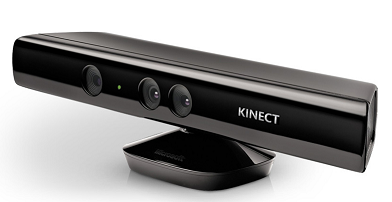
\includegraphics[width=0.3\textwidth]{image/kinect_camera.png}
  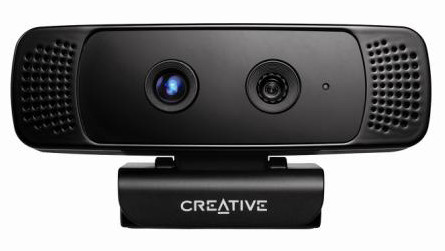
\includegraphics[width=0.3\textwidth]{image/intel_creative_camera.jpg}}
  \caption{Kinect, da Microsoft, e a câmera da \textit{Creative} com parceria da Intel}
  \label{fig:depth_camera}
\end{figure}

O uso de câmeras em carros e caminhões também tem aumentando nos últimos anos. Sistemas de segurança capazes de verificar se o motorista esta saindo indevidamente da faixa, ou se o veículo esta em rota de colisão com algum outro automóvel ou objeto e até mesmo monitorando o stress do motorista já são comuns em vários modelos de veículos. Mas pouco vimos o uso dessas câmeras para interação do motorista com a grande quantidade de controles que temos nos carros. Aumentar ou diminuir o volume do rádio, trocar de faixa de música, dar zoom no mapa do sistema de navegação são alguns exemplos de comandos que poderia ser dados por meio de gestos.
O sistema de gestos também pode ser usado como um complemento ao sistema de reconhecimento de voz, bastante comum hoje nos carros.

\section{Objetivo}

O objetivo do trabalho é discutir as principais técnicas para reconhecimento de gestos e poses de mão em um ambiente automotivo.
Os algoritmos e metodologias hoje utilizados para segmentar e extrair características de imagens e vídeos devem ser estudados e verificados se atingem seu propósito em um ambiente automotivo.
As características extraídas são utilizadas como entrada em um classificador, responsável por reconhecer gestos e poses de mão, e assim, permitir uma interação com o veículo traduzindo os gestos em comandos para o carro.

\section{Justificativa}

Esse ambiente apresenta uma forte variação de luz e ausência de controle nas características da mão e do braço do motorista (cor de pele, braço com ou sem vestimentas e vestimentas de cores e estampas diferentes). 

As condições gerais dentro do automóvel inclui uma grande variação de iluminação, mudança de usuário e fundos não uniformes. Além disso, a aceitação do usuário é um item bastante importante, portanto coisas como uma iluminação artificial visível, restrição de vestimentas e calibração extensiva não pode ser tolerados. Tento isso em mente, alguns critérios e requisitos para o sistema podem ser estabelecidos:

\begin{itemize}
\item robustez contra ambientes ruidosos
\item iluminação invisível
\item independente de usuário
\item sem calibração ou treinamento pelo usuário
\item pequeno e compreensível conjunto de gestos
\item reação do sistema com o mínimo de latência
\end{itemize}

\section{Hipótese}

As metologias apresentadas para a segmentação, extração de características e classificação precisam ser estudas e implementadas para verificar se o processamento requerido viabiliza o seu uso em uma área aonde o custo é relativamente sensível.

\section{Metodologia}

A metodologia do projeto abrange todas as principais etapas de um problema de visão computacional, com a captura da imagem, segmentação, extração de características, reconhecimento de padrões e interpretação dos resultados obtidos.

Na etapa de captura da imagem, os artigos \cite{ref2} e \cite{ref1} fazem uso de uma câmera infravermelha simples, onde o ambiente é iluminado por infravermelho de curta distância (950nm). A câmera ainda possui um filtro de luz, permitindo apenas que a luz infravermelha seja capturada pela câmera. Apesar de existir câmeras mais sofisticadas, optamos por usar a câmera mais simples, em vez das câmeras de profundidade por ser mais compatível com os padrões de mercado automotivo. No momento que esse texto foi escrito, as câmeras de profundidade ainda possuem um preço proibitivo e a quantidade de processamento é bastante limitada em um ambiente embarcado. Uma outra razão para a escolha de uma câmera mais simples se dá ao fato que não pretendemos estudar nesse texto os processos de segmentação de imagem. Vamos considerar que esse problema esteja resolvido e vamos nos concentrar em como melhor representar e classificar as poses e gestos de mão.

As imagens de poses e os vídeos dos gestos serão obtidos em  dois ambientes distintos. Primeiro em um ambiente controlado com fundo homogêneo de cor preta e em uma sala totalmente escura (essa base de dados será usada como referência para os algoritmos implementados). O outro será obtido no interior de um veículo, tanto de dia como de noite.
Se usássemos uma câmera de profundidade, a segmentação seria simplesmente pela distância da mão à câmera. Mas como vamos usar uma câmera normal, vamos usar dois tipo de segmentação diferente. 
Para as imagens com fundo controlado, vamos usar um threshold global como método para separar o fundo. Nas imagens no carro, vamos usar os algoritmos de remoção de fundo, usando um frame de calibração.
Grande parte dos artigos sobre reconhecimento de mãos utilizada a cor da pele como segmentação. Aqui não temos essa opção pois a câmera infravermelha não tem as informações de cor.

Depois da etapa de segmentação, vem a etapa de extração de características e é nessa etapa que vamos focar nossos estudos. Os artigos \cite{ref2} e \cite{ref1} utilizam os momentos Hu como vetor de características para poses de mão.
Um dos precursores em extração de características da mão usando histograma de orientação de gradientes (HOG) foi o laboratório da Mitsubishi que publicou um conjunto de artigos \cite{ref3}, \cite{ref4} sobre o tema. Nesses artigos foi feito o HOG da imagem como um todo, em tons de cinza, e dividindo os ângulos em 36 grupos. O método não era geral o suficiente para ser usado com um algoritmo válido para representação de uma forma genérico e por isso, o mesmo evolui para o SIRF. Acontece que a aplicação é bastante parecida com a proposta desse trabalho e por isso HOG é melhor detalhado posteriormente.

Os classificadores mais utilizados na literatura existente serão avaliados, para que se conheça sua performance em relação a tempo de processamento e acerto. Desse estudo serão terminados os classificadores mais adequados para a aplicação proposta.

\section{Organização da dissertação}

\todo{Elaborar no final}

